\section{Comparación}
	
	Ahora lo que nos interesa es comparar los 2 algoritmos descriptos anteriormente. La idea de esto es ver como se comportan las podas frente a no tener podas. Para esto tomamos los tiempos de ambos algoritmos sobre la entrada random descripta en las secciones anteriores. La razón por la cuál optamos por la entrada random es porque nos parece el mejor caso para comparar los algoritmos, ya que no podemos saber que se está podando y que no. Y, además, según lo que vimos antes es un mal caso para las podas, mientras que no es un caso tan malo para la versión sin podas. 

\begin{figure}[h]
\begin{subfigure}{0.5\textwidth}
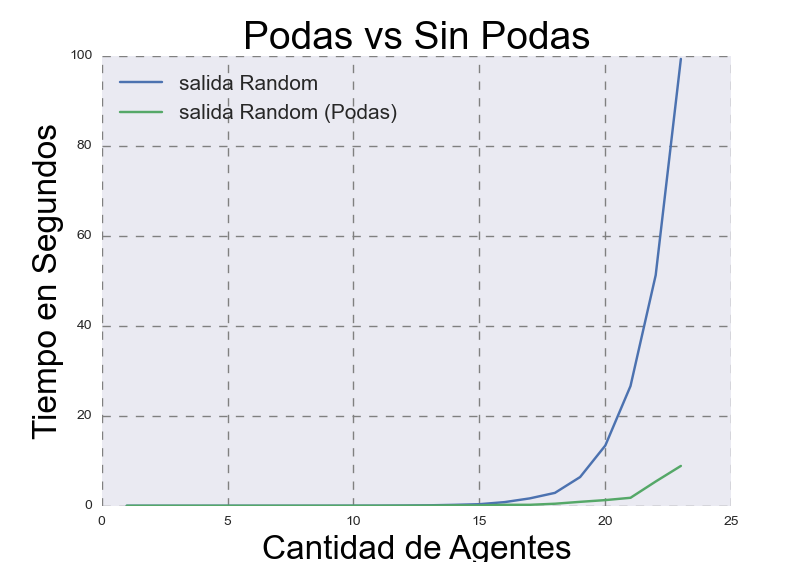
\includegraphics[scale=0.45]{Vs.png}
\end{subfigure}
\end{figure}

\begin{figure}[h]
\begin{subfigure}{0.5\textwidth}
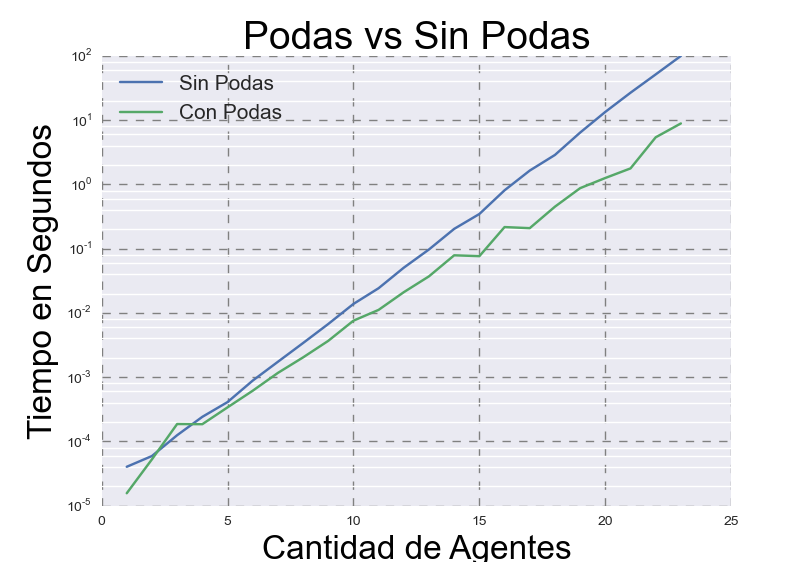
\includegraphics[scale=0.45]{VsLog.png}
\end{subfigure}
\end{figure}
	
	Lo que podemos ver en los gráficos es que el algoritmo con podas es más rápido que el que no tiene podas. Esto se debe a que las podas me ahorran recorrer ramas que no van a aportar una mejor solución al problema y, además, cuando hacemos el chequeo de si un agente es confiable, las podas hacen un chequeo más profundo que la versión sin podas.   

	